\documentclass[]{article}

\usepackage{graphics}
\usepackage{amsmath,amssymb,wasysym}
\usepackage{bm}
\usepackage{natbib}
\usepackage{textcomp}
\usepackage{derivative}
\usepackage{caption}
\usepackage{hyperref}
\usepackage{authblk}

\usepackage{graphicx}
\graphicspath{ {./figs/} }

%opening
\title{Some notes on Bayesian nonnegative matrix factorisation}
\author{Shota Gugushvili}
\affil{Biometris, Wageningen University \&\ Research}

\begin{document}

\maketitle

\begin{abstract}
These notes provide some information on Bayesian non-negative matrix factorisation. 
\end{abstract}

\section{Introduction}

These notes provide some information on PCA and Bayesian non-negative matrix factorisation. They are partly based on Hendrik Steinbach's master thesis ``Matrix factorization techniques for dimensionality reduction and clustering: a comparative study in genomics". Hendrik wrote the thesis at Leiden University and WUR under Fred van Eeuwijk's and my supervision. In order to stay on the didactic side, notes do not go into full details and extensive comparisons. They do contain references to the literature. Description of the singular value decomposition and PCA is just enough to understand similarities to and differences from non-negative matrix factorisation. Knowledge of their other properties is tacitly assumed.

\section{Generalities}

Given is a data matrix $Y$ of dimensions $U \times I$. Think of $U$ as a number of subjects and $I$ as a number of variables\footnote{Notation comes mostly from \citet{kucukelbir2017} and might not be ideal, but I left it as such. For instance, $U$ stands for users and $I$ stands for items: the original application there was the movie ratings dataset.}. The $u$th row of $Y$ is an observation vector for the $u$th subject. The $i$th column contains the $i$th variable values.

I aim at extracting signal $\Lambda$ from noisy observations $Y$. The matrix $\Lambda$ has the same dimensions as $Y$. A schematic picture is given in Figure \ref{fig:signal_in_noise}.

\begin{figure}[h]
	\centering
	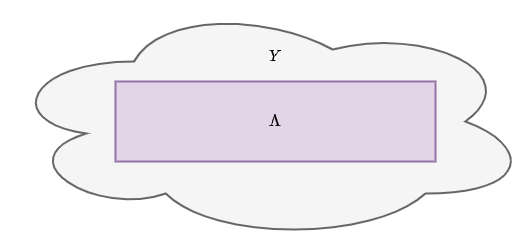
\includegraphics[width=8cm]{signal_in_noise.png}
	\caption{Schematic depiction of signal $\Lambda$ within noisy observations $Y$.}
	\label{fig:signal_in_noise}
\end{figure}

The signal $\Lambda$ is assumed to be low-rank, as detailed next. Consider a typical situation in modern applications, where the number of subjects is smaller than the number of variables: $U < I$ (often $U \ll I$). Assuming that there are no linear dependencies among the rows of $Y$, the rank of $Y$ is $\min(U, I) = U$. A low-rank approximation to $Y$ is
\begin{equation}
\label{factorisation}
\Lambda = \Theta \times B.
\end{equation}
Here $\Theta$ is $U \times K$-dimensional with $K < I$, while $B$ is $K \times I$-dimensional. See Figure \ref{fig:nmf} for a visualisation of a relationship between various matrices at hand. The rank of $\Lambda$ is at most $K$, and we know $K < U$. Typically one chooses $K$ such that
\[
K  (U + I) < U  I.
\]
This ensures that the matrices $\Theta$ and $B$ combined have less entries than the matrix $\Lambda$. Thereby less free parameters are needed to describe $\Theta$ and $B$ than a totally unstructured $\Lambda$ would require.

Columns of matrix $\Theta$ can be thought of as latent meta-variables. Rows of matrix $B$ give a basis in which these meta-variables are expressed. A single row of matrix $\Lambda$ is a linear combination of the rows of matrix $B$, where weights come from the columns of matrix $\Theta$; see Figure \ref{fig:nmf3}.

\begin{figure}[h]
	\centering
	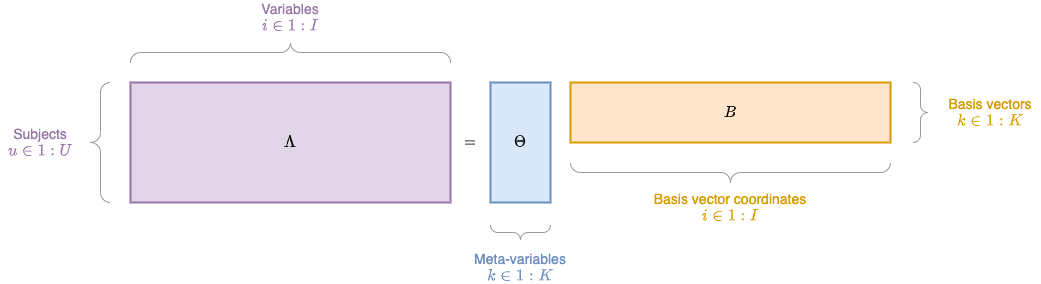
\includegraphics[width=12cm]{NMF.png}
	\caption{Schematic depiction of the relationships between matrices $\Lambda$, $\Theta$ and $B$.}
	\label{fig:nmf}
\end{figure}

\begin{figure}[h]
	\centering
	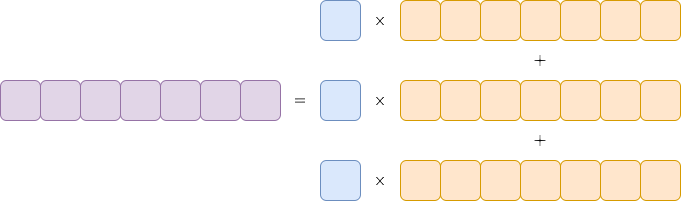
\includegraphics[width=12cm]{NMF3.png}
	\caption{Each row of matrix $\Lambda$ is a linear combination of the rows of basis matrix $B$ with weights from columns of matrix $\Theta$.}
	\label{fig:nmf3}
\end{figure}

In the audio signal processing literature the matrix $Y$ is a spectrogram, $B$ is a codebook of spectra consisting of basis vectors, while $\Theta$ is a matrix of their gains in each frame; see, e.g., \citet{virtanen2008}.

Matrix $\Theta$ can be used to study patterns in the data and for clustering. A low-rank representation aids in that. Feature engineering is another natural application.

\section{SVD and PCA}

SVD gives
\[
Y = \mathcal{U} \times \Sigma \times \mathcal{V}^T.
\]
Here the matrix $\Sigma$ is the diagonal matrix of singular values of $Y$ in decreasing order, $\mathcal{U}$ is the matrix of the corresponding left singular vectors of $Y$ and $\mathcal{V}$ is the matrix of the right singular vectors. Matrices $\mathcal{U}$ and $\mathcal{V}$ have orthonormal columns. The main diagonal of the matrix $\Lambda,$ on the other hand, has positive entries. See \citet{strang2000}, Section 7.2.

A low-rank approximation to $Y$ is obtained by retaining the first $K$ columns of $ \mathcal{U}$ and $ \mathcal{V}$, and the upper-left $K \times K$ part of $\Sigma$,
\[
\Lambda =  \mathcal{U}_K \times \Sigma_K \times \mathcal{V}_K^T,
\]
see \citet{murphy2022}, Section 7.5.5. The Eckart-Young-Mirsky theorem states that this $\Lambda$ gives the lowest reconstruction error in the Frobenius norm over all matrices $X$ of rank $K$:
\[
\Lambda = \operatorname*{arg\, min}_{X : \operatorname{rank}(X)=K} \| Y - X \|_F.
\]
See \citet{strang2000}, page 393. There are various ways in which the Frobenius norm can be introduced, but for now it is enough to say that it is the square root of the sum of the squared entries of a matrix.

To link SVD to \eqref{factorisation}, set $\Theta = \mathcal{U}_K \times \Sigma_K$ and $B = \mathcal{V}_K^T.$

Finally, the relationship of SVD to PCA is as follows: assume $Y$ is centred (this is essential). Then the columns of the matrix $\mathcal{U} \times \Sigma$ are principal components or scores, while the columns of $\mathcal{V}$ are principal axes. Furthermore, the standardised scores are given by columns of $\sqrt{U-1} \cdot \mathcal{U}$, while loadings are the columns of $\mathcal{V}\Sigma/\sqrt{U-1}$. See \citet{murphy2022}, page 659 for details and further pointers.

SVD is a modern way of performing the PCA decomposition\footnote{Traditionally, PCA has been done via spectral decomposition (eigendecomposition) of the sample covariance or correlation matrix. However, forming the sample covariance matrix when the number of features is large is costly, and furthermore, SVD yields numerically more stable computations. Cf. \citet{ripley1996}, page 290. Thus, \texttt{prcomp} in {\bf R} relies on SVD, while \texttt{princomp} follows an older route for compatibility with S-PLUS. PCA in {\bf scikit-learn} in {\bf Python} is implemented through SVD and randomised truncated SVD.}.

There are probabilistic and Bayesian reformulations of PCA, but I will not consider them here. See, e.g., Section 12.2 in \citet{bishop2006} for details.

\section{NMF}

Assume $Y$ has non-negative entries (this is important), but otherwise they are allowed to be integer- or real-valued. There are two commonly used versions of NMF. Either assumes the matrices $\Theta$ and $B$ in \eqref{factorisation} to have non-negative entries. One possibility is that the pair $(\Theta, B)$ is a minimiser of the criterion $\| Y - X  \|_F$
over $X$ such that $X=W \times H$ for $W$ and $H$ with non-negative entries. This is least squares estimation of an approximating $\Lambda$, subject to the stated constraints on $\Theta$ and $B$.

Another possibility is to maximise the criterion
\begin{equation}
\label{poisson_crit}
\sum_{u=1}^U \sum_{i=1}^I \left[  Y_{ui} \log(W \times H)_{ui} - (W \times H)_{ui}  \right]
\end{equation}
subject to non-negativity constraints on the entries of $W$ and $H$. If $Y$ were integer-valued, this would amount to a Poisson generative model for $Y$, i.e.
\[
Y \sim \operatorname{Poisson}(\Lambda),
\]
and maximisation of the corresponding log-likelihood $\ell_Y(X)$ over matrices $X$ subject to the constraint $X=W \times H$ for $W$ and $H$ with non-negative entries. Cf.\ \citet{lee1999}. An iterative algorithm for non-negative matrix factorisation from \citet{lee1999} reduces to the EM algorithm; this can be shown by examining the equations for the E and M steps, see \citet{cemgil2009}. Strengths and limitations of the EM algorithm are part of the statistical folklore.

There are no further restrictions on $\Theta$ and $B$ except non-negativity of their entries. This is unlike SVD/PCA. However, both methods try to solve a matrix approximation problem.

When further restrictions are imposed on the factors in the decomposition, links with various clustering algorithms emerge; see \citet{ding2005}. For instance, the $K$-means algorithm can be recovered. However, introducing extra (non-linear) constraints is not necessarily the best strategy to proceed with matrix factorisations from the numerical point of view.

NMF has some Bayesian roots, see \citet{richardson1972}.

\section{Benefits of NMF}

PCA has been widely used in, e.g., social sciences, but has found a limited use in natural sciences (\citet{paatero1994}). The reason is the non-negativity constraint, which is natural in many physical problems. For instance, there cannot be a negative amount of a basic constituent in any sample, nor can the composition of any basic constituent contain a negative percentage of any element; see \citet{paatero1994}, page 112. PCA cannot guarantee non-negativity of the matrix decomposition, while this property is built into NMF.

\citet{paatero1994}, page 120, argue that orthogonality in matrix decompositions is irrelevant in physical sciences. PCA delivers orthogonality, while it is in general precluded by the non-negativity constraint.

\citet{lee1999} illustrate and contrast performance of NMF and PCA on image data. According to them, the non-negativity constraints are compatible with the intuitive notion of combining parts to form a whole, which is how NMF, they say, infers a parts-based representation\footnote{Later work has shown that parts-based representations are not always automatically delivered by NMF. However, this can be achieved with some suitable modifications of the basic algorithm; see, e.g., \citet{hoyer2004}.}, as it focusses on learning localised features in the data. This is not possible with PCA.

NMF often delivers already quite sparse solutions in those situations where PCA does not. Sparsity helps with interpretability, and sparse solutions fed into other procedures often give better practical results than non-sparse ones. Think of clustering algorithms: it is easier to differentiate cases where only a few components are large, as it is less likely that different clusters have the same components large. Obviously, there exist also sparse versions of PCA. But these are non-trivial extensions computationally, whereas the basic SVD algorithm is straightforward.

Where the uses of PCA have outweighed those of NMF, this seems to an extent a consequence of inertia in those fields.

\section{Bayesian NMF}

Bayesian NMF postulates a parametric data generation mechanism. Model parameters are equipped with priors. Inference is based on the posterior distribution of the parameters.

A parametric statistical model for Bayesian NMF from \citet{virtanen2008} and \citet{cemgil2009} assumes 
\[
Y \sim \operatorname{Poisson}(\Lambda),
\]
for $ \Lambda = \Theta \times B$. This notation has to be understood entry-wise. It is assumed that the entries of $Y$ are non-negative integers (note that restriction to integers is not necessary for optimisation of expression \eqref{poisson_crit}). Other possibilities for the likelihood are, e.g., a binomial likelihood or a Gaussian likelihood (cf. \citet{mnih2007}).

A Bayesian model is obtained from this parametric model by imposing priors on $\Theta$ and $B$. There are various possibilities. Earlier works focussed on Gamma priors due to the well-known Poisson-Gamma conjugacy property. This came in handy in the Gibbs sampler and the coordinate ascent variational inference; see \citet{cemgil2009}. However, with the advent of modern Bayesian software such as {\bf{Stan}}, see \citet{carpenter2017} and \citet{stan2024}, conjugacy is thought of being less important. Furthermore, a sequential nature of coordinate updates in the Gibbs sampler and the coordinate ascent variational inference, and possible strong correlations between latent variables\footnote{Signals are structured.} renders these methods inherently slow for modern applications focussing on big data; cf. \citet{blei2017}, page 869 and \citet{lindsten2013}, Section 1.3.

I will bypass conjugacy altogether\footnote{For non-Bayesians this should lift a veil of mystery from the use of the Gamma prior in this setting.}. The following two properties are required from the prior: act as a reguliser for numerical stability of computations, and encourage sparse representations of the signal.

I start with the prior on $B$, which is defined as
\[
B_{ki} \sim \operatorname{Exponential}(1)
\]
for $k=1,\ldots,K$ and $ i = 1,\ldots , I.$ The scaling of the prior is immaterial, in that it gets compensated by the multiplicative nature of decomposition \eqref{factorisation} through matrix $\Theta$. Here the scale parameter is set to $1$ for convenience. The prior ensures positivity of the entries of $B$. There is no specific structure assumed about the basis vectors, though it may be present in some applications. When such a structure is present, it can be built into the prior, but this has to be done on a case-by-case basis. Using the exponential prior is like using the $L_1$-penalty on the entries of the matrix $B$ coupled with non-negativity.

The prior for $\Theta$ uses a more involved construction. In practice the number $K$ of the required meta-variables is often unknown. Automatic Relevance Determination (ARD) that was first proposed in the context of neural networks by MacKay and Neal (see \cite{mackay1995}) is a simple, yet efficient strategy to address this issue; cf. \citet{bishop2006}, page 582. This method starts with taking $K$ large for a given application. It then requires using a different shrinkage parameter per each column of $\Theta$ that effectively switches it off, should the column turn out to be superfluous. In practice the method may overshrink some columns relative to others. This behaviour can be repaired by using a global shrinkage parameter that acts on the entire matrix $\Theta.$ At the same time, as its name suggests, this parameter promotes sparsity throughout the entire matrix $\Theta$. Figure \ref{fig:ARD} may help in understanding the main ideas. ARD is computationally more convenient than equipping the number of meta-variables $K$ with a prior. The latter leads to a family of models with varying dimensions, inference for which is computationally challenging; see \citet{green95} and \citet{godsill2001}. ARD deals with a model of fixed dimension, but has a built-in ability of essentially turning off the surplus dimensions.

\begin{figure}[h]
	\centering
	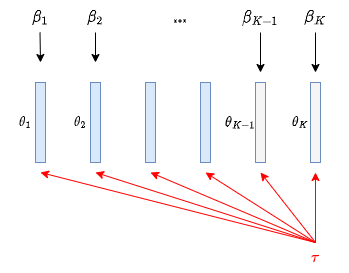
\includegraphics[width=8cm]{ARD.png}
	\caption{Schematic depiction of ARD for NMF. Columns of matrix $\Theta$ are denoted by $\theta_k$. Here the last two columns are superfluous, which is indicated by their lighter colouring. Shrinkage parameters $\beta_k$ act on individual columns $\theta_k$. The global shrinkage parameter $\tau$ acts on the entire matrix $\Theta$.}
	\label{fig:ARD}
\end{figure}

The exact details of the construction are as follows: at the lowest level,
\[
\theta_{uk} \sim \operatorname{HalfNormal}(0, \tau \beta_k)
\]
for $u=1,\ldots,U$ and $ k = 1,\ldots , K.$ Here $ \operatorname{HalfNormal}(0, \tau \cdot \beta_k)$ stands for Normal distribution with mean $0$ and standard deviation $\tau \cdot \beta_k$, and constrained to be positive. The parameter $\tau$ is the global shrinkage parameter, while $\beta_k$'s are the local shrinkage parameters. Small values of $\tau$ and $\beta_k$'s correspond to greater degree of shrinkage.

In the next layer of hierarchy,
\[
\beta_k \sim \operatorname{HalfStudent}(3, 0, 5)
\]
for $k=1,\ldots,K$, and
\[
\tau \sim \operatorname{HalfStudent}(3, 0, 5).
\]
Here $ \operatorname{HalfStudent}(3, 0, 5)$ stands for Student distribution with 3 degrees of freedom, location $0$ and scale $5$, and constrained to be positive. Hyperparameters of the priors are not carved in stone and may be modified as required in specific applications. The whole construction is somewhat inspired by the horseshoe prior; see, e.g., \citet{carvalho2009}. Heavy-tailed priors like Student have better shrinkage properties than the light-tailed ones (like Gaussian)\footnote{See \citet{carvalho2009}, or \url{https://www.stephanievanderpas.nl/shrinkage-priors} for relevant references dealing with theory.}. There is no direct analogue of these priors among the $L_p$ penalisation methods.

%The graphical model is in Figure \ref{fig:graph_model}.

Aggregate all the parameters and latent variables of the Bayesian model into $Z$. Bayes' theorem gives the posterior density
\begin{equation}
\label{bayes}
p(Z|Y) = \frac{p(Y|Z)p(Z)}{\int p(Y|Z)p(Z) \odif{Z}}.
\end{equation}
Posterior can then by used to obtain point estimates of $\Theta$ and $B$, and to conduct inference.

The hyperparameters $\beta_k$ can be thought of as a rough analogue of the singular values in SVD/PCA. Their posterior point summaries (means or medians) can thus be used to rank meta-variables in order of their importance.

My final remark concerns identifiability. The Bayesian model above is not identifiable, in that swapping columns in $\Theta$ together with corresponding rows in $B$ leads to the same product $\Lambda$, and hence the same log-likelihood. A consequence of that is a multimodal posterior. Various solutions to fix the identifiability issue in Bayesian factor models are discussed in \citet{murphy2022}, Section 20.2.4; cf.~also \citet{kucukelbir2017}. I will use none out of purely practical considerations: firstly, they incur additional computational cost. Secondly, they are not necessarily natural restrictions in every application. Thirdly, my engine to compute approximate posterior will be variational inference with a unimodal family of approximating distributions. The variational density in such cases locks into one of the posterior modes due to special properties of the variational criterion, see \citet{bishop2006}, page 469. The latter is enough for my purposes. Which mode is selected depends on the initialisation of the algorithm.

\section{Benefits of Bayesian approach}

Bayesian approach solves the problem of choosing the number of meta-variables $K$. It allows an intuitive specification of sparsity degree of the signal through a suitable choice of prior distributions. Arguments for advantages of sparse coding of a signal in, e.g., sensory systems are given in \citet{field1994}, and conform to the intuition that, e.g., natural images may generally be described in terms of a small number of structural primitives, such as edges or lines; see \citet{olshausen1997}, page 3315. Even if appealing to sensory systems is not fully convincing, sparse coding represents a useful first approximation. NMF in its basic form does not always automatically deliver a good parts-based representation of the signal (see \citet{hoyer2004}, page 1460), but this can be encouraged through the use of prior distributions. Sparsely coded signals are more amenable to inferring hidden structures in the data: for such signals only a few basis vectors are active at a time, and qualitatively different signals have a greater chance of having different components active, and thus being distinguishable. Bayesian priors are more flexible tools than the commonly used $L_p$ penalisation methods. Moreover, a Bayesian approach also allows an extension of the basic NMF model to a probabilistic mixture of NMF models. This is an attractive alternative to non-linear modelling (e.g., Self-Organizing Maps). Finally, a Bayesian approach can also handle missing data without need of an imputation algorithm. I will not consider this here.

\section{Variational inference}

The marginal likelihood or the evidence
\[
\int p(Y|Z)p(Z) \odif{Z}
\]
in \eqref{bayes} is intractable, and hence posterior is not readily accessible. Therefore an approximation method has to be used. MCMC is not scalable in the present context; cf.\ \citet{kucukelbir2015} and \citet{kucukelbir2017}. Instead I will use variational inference to approximate the posterior. This converts the problem of finding the approximate posterior into an optimisation task. The variational objective called the evidence lower bound (ELBO) does not involve the untractable marginal likelihood. The key ideas are explained in Figure \ref{fig:VI2}. Further details are given, e.g., in \cite{bishop2006}, Chapter 10, or \citet{murphy2023}, Chapter 10. A recent overview article is \citet{blei2017}. Variational inference has its roots in statistical physics, where the method is used to approximate the distribution of a system by minimising the variational free energy; see \cite{mackay2003}, Chapter 33.

There are various algorithmic realisations of variational inference. I will employ the automatic differentiation variational inference as implemented in {\bf Stan}; see \citet{kucukelbir2015} and \citet{kucukelbir2017}.

\begin{figure}[h]
	\centering
	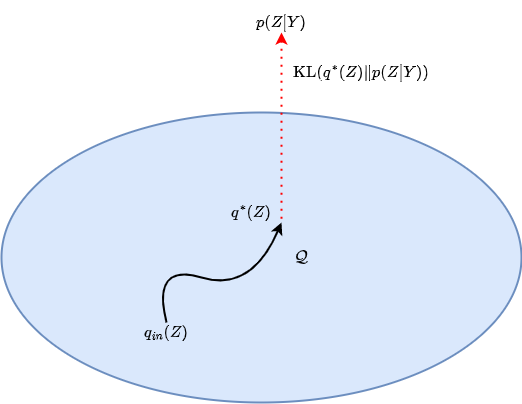
\includegraphics[width=8cm]{VI2.png}
	\caption{Schematic depiction of variational inference. The intractable posterior density $p(Z|Y)$ lies outside of the tractable approximating family $\mathcal{Q} = \{ q(Z) \}$. Variational inference proceeds from the initial approximation $q_{ini}(Z)$ and iteratively improves upon it through optimising the evidence lower bound (ELBO). The iterative process is stopped once  arriving at the optimal solution $q^{\star}(Z)$. This optimal solution minimises the Kullback-Leibler divergence between the family $\mathcal{Q}$ and the posterior $p(Z|Y)$.}
	\label{fig:VI2}
\end{figure}

ADVI starts by internally transforming the constrained latent variables to the real coordinate space, while leaving unconstrained variables unchanged. In the real coordinate space, it postulates a Gaussian approximating family to the posterior. The user has a choice between a Gaussian with a diagonal covariance matrix, and a Gaussian with a general covariance matrix. The former case is referred to as the mean-field inference, while the latter as the full-rank inference. The full-rank Gaussian family is more flexible, while the mean-field family leads to faster computations and often yields numerically more stable runs. The mean-field family takes its name from the mean field theory in physics, which is a special case of a general variational free energy approach of Feynman and Bogoliubov (see \citet{mackay2003}, page 422). Optimisation of the variational objective in ADVI is performed through stochastic gradient descent (SGD) and relies on automatic differentiation (AD) for fast gradient evaluations. Once a (local) optimum has been found, a sample of a given size is drawn from the variational density and back-transformed to the constrained latent space. This enables quick summarisation and plotting of inference results\footnote{Technically, the entire variational density is available analytically. But when the number of latent variables is large (which is raison d'\^{e}tre of the variational approach in the first place), it is a cumbersome object to manipulate. On the other hand, a sample from the variational density is easier to handle in inferential, summarisation and visualisation tasks.}. On the other hand, with a large number of latent variables, the storage might become an issue (my experience). There are several user-defined tuning parameters in ADVI, but the default choices often work well and provide a natural starting point. It is probably a good practice to run the algorithm several times to assess stability of the obtained results.

Advantages of ADVI include speed, scalability, and its essentially automatic nature. A disadvantage is that the method is approximate and cannot recover the exact posterior distribution in the limit when the number of iterations is taken to infinity. In particular, even if the centre of the posterior distribution is well-approximated, the method may underestimate its spread, and hence inferential uncertainty; see, e.g., \cite{bishop2006}, page 467. Gaussian approximation might be too crude as a distributional assumption in some situations. If the goal is recovery of the centre of the posterior distribution, with some (possibly crude) measure of uncertainty, variational inference is typically fine.

\section{Bayesian NMF via ADVI}

I provide an implementation of the Bayesian NMF model via ADVI in {\bf Stan}. To that end it is enough to specify relationships between various variables defing the model, while the inference itself takes place under the hood. This is probabilistic programming, see \citet{carpenter2017}. There is no need to derive manually the iterative update equations for the variational density. {\bf Stan} is the most widely used general-purpose software for Bayesian computations; see \citet{strumbelj2024}.

The starting point of the implementation was the one proposed in Figure 19 in \citet{kucukelbir2017}, but this was radically modified, e.g., via incorporating ARD and dropping the identifiability constraint (which proved to cause numerical problems, when I experimented with it). Priors in general are different.

\section{Simulated data example}

Here is a simulated data example. The meta-variable matrix $\Theta$ is $60 \times 3$-dimensional. The basis matrix $B$ is $3 \times 900$-dimensional. This gives a $60 \times 900$-dimensional signal matrix $\Lambda$, that serves as a mean matrix for the Poisson-distributed observation matrix $Y$.

The matrix $\Theta$ has roughly a block-diagonal structure: large entries appear in 3 blocks along the main diagonal, while other entries are small. See Figure \ref{fig:theta} for a visualisation. A similar structure is assumed for the matrix $B$. Details can be found in the accompanying computer code, for visualisation of $B$, $\Lambda$ and $Y$ see Figures \ref{fig:B}, \ref{fig:lambda} and \ref{fig:Y}. Some structure in matrix $Y$ is apparent to the bare eye. The main interest lies in recovering the structure of matrix $\Theta.$

\begin{figure}
	\centering
	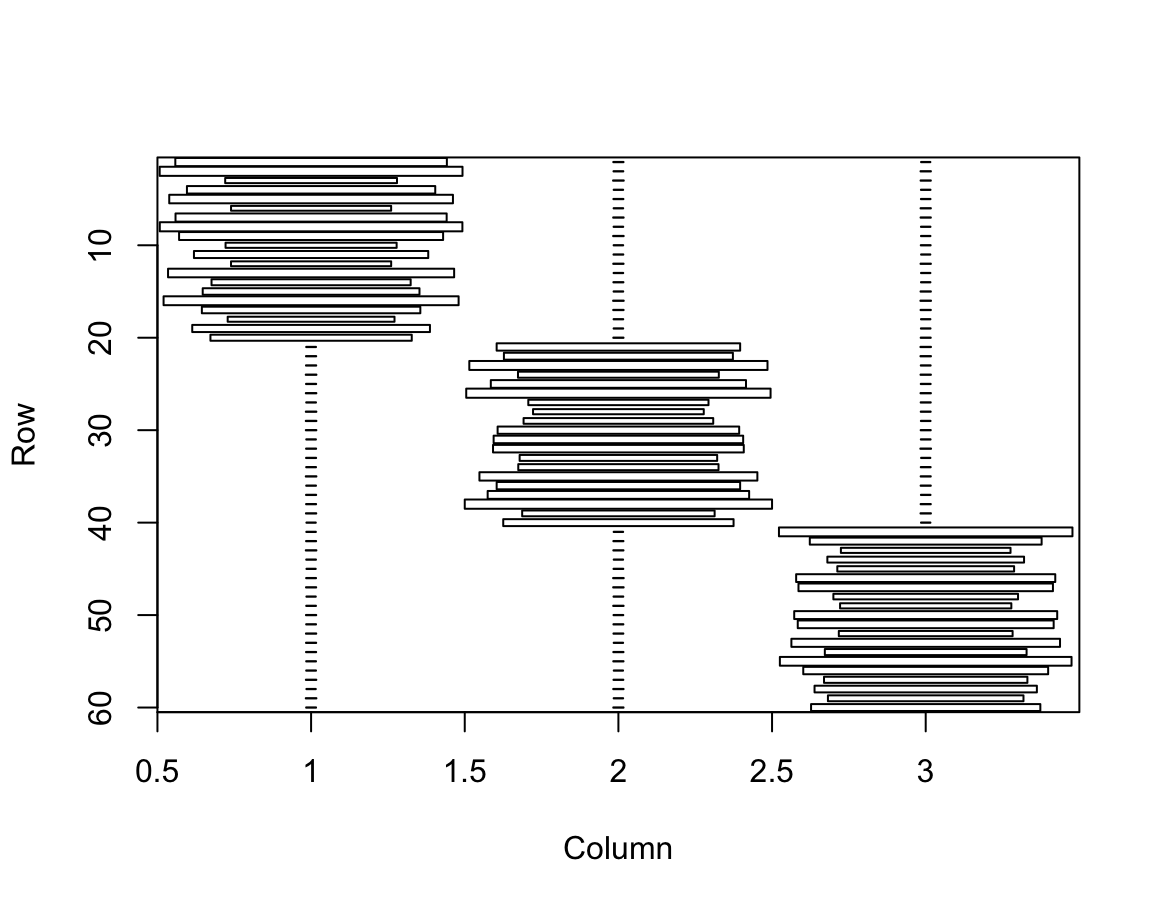
\includegraphics[width=8cm]{theta.png}
	\caption{Hinton diagram for matrix $\Theta$. The box sizes represent the relative sizes of the corresponding matrix entries.}
	\label{fig:theta}
\end{figure}

\begin{figure}
	\centering
	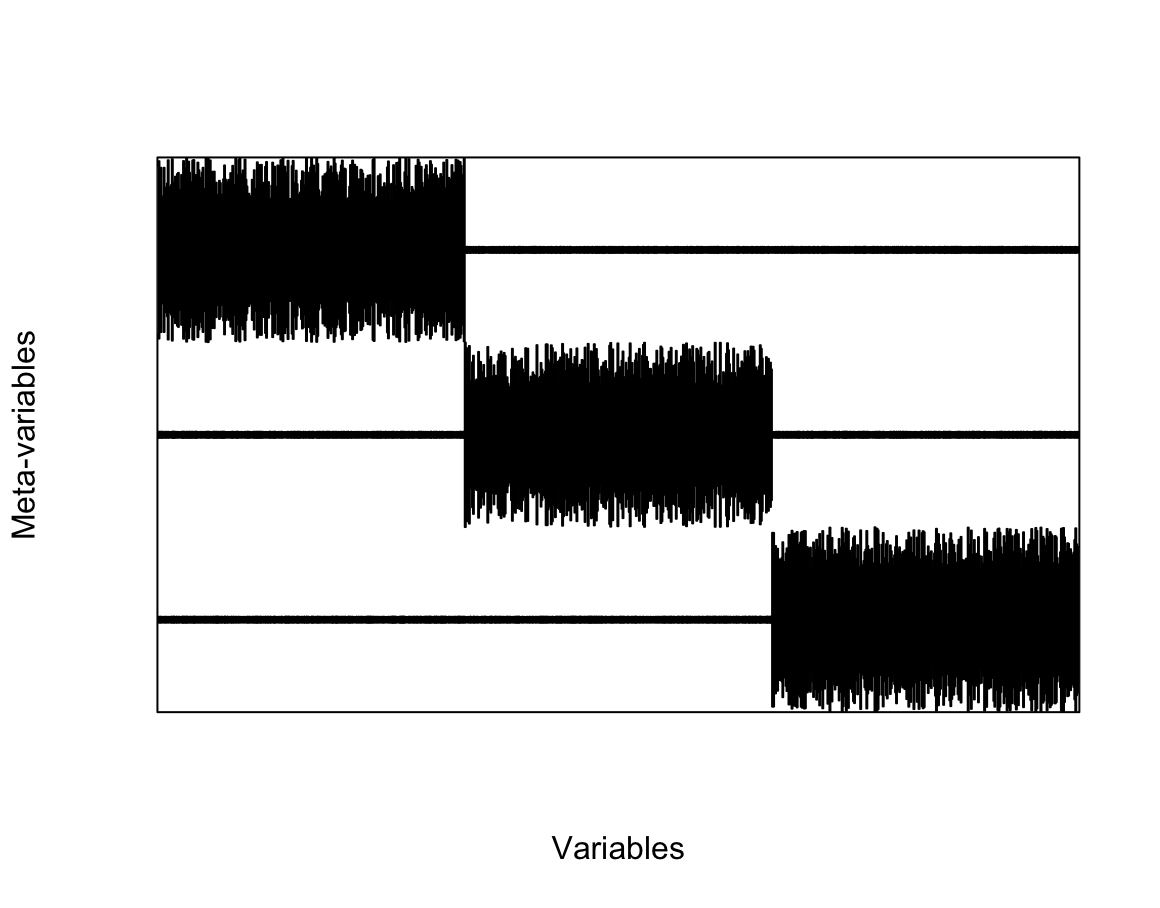
\includegraphics[width=8cm]{b.png}
	\caption{Hinton diagram for basis matrix $B$.}
	\label{fig:B}
\end{figure}

\begin{figure}
	\centering
	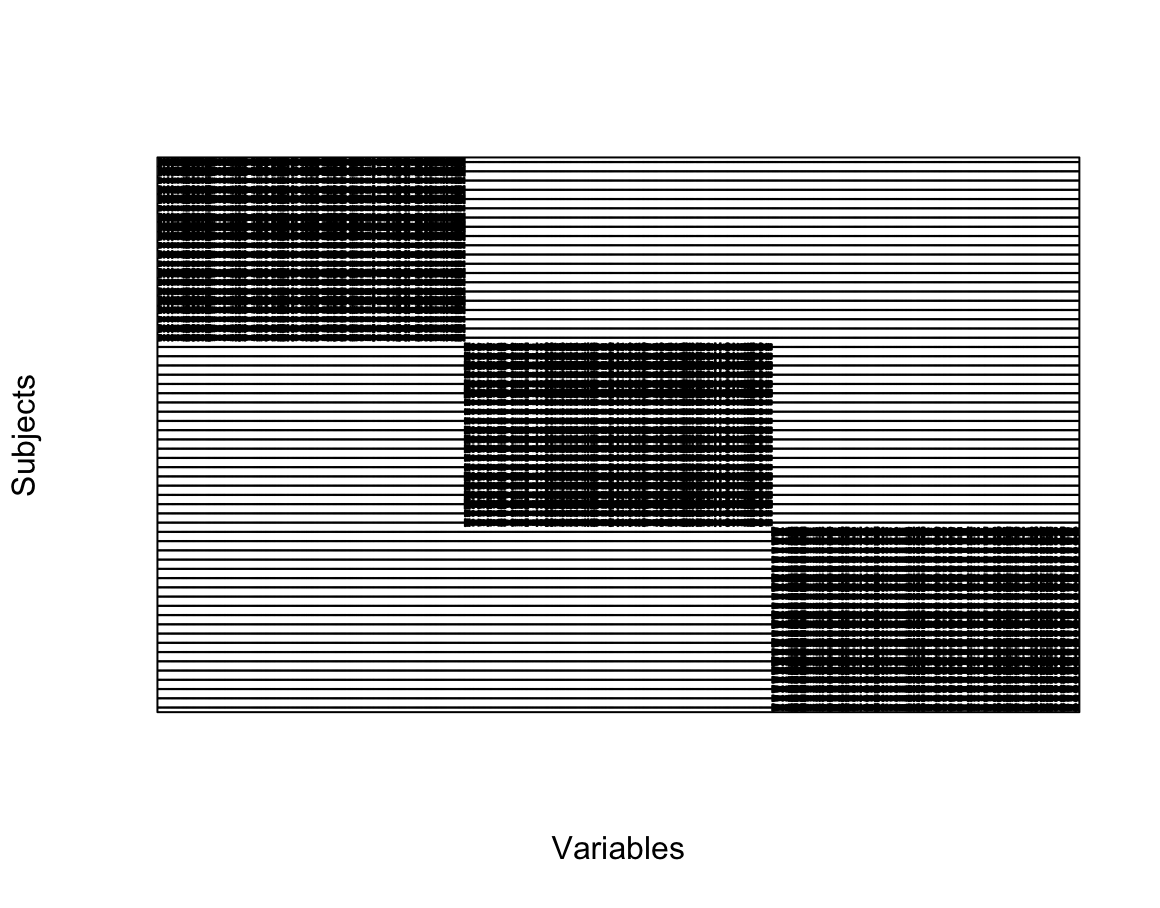
\includegraphics[width=8cm]{lambda.png}
	\caption{Hinton diagram for signal matrix $\Lambda$.}
	\label{fig:lambda}
\end{figure}

\begin{figure}
	\centering
	\includegraphics[width=8cm]{Y.png}
	\caption{Hinton diagram for observation matrix $Y$.}
	\label{fig:Y}
\end{figure}

Bayesian NMF was performed assuming $K=5$ latent dimensions. Two dimensions are thus superfluous. The posterior median for $\Theta$ is shown in Figure \ref{fig:theta_hat}. The structure recovery is excellent, as seen from comparison to Figure \ref{fig:theta}. The 2 surplus dimensions are essentially switched off.

\begin{figure}
	\centering
	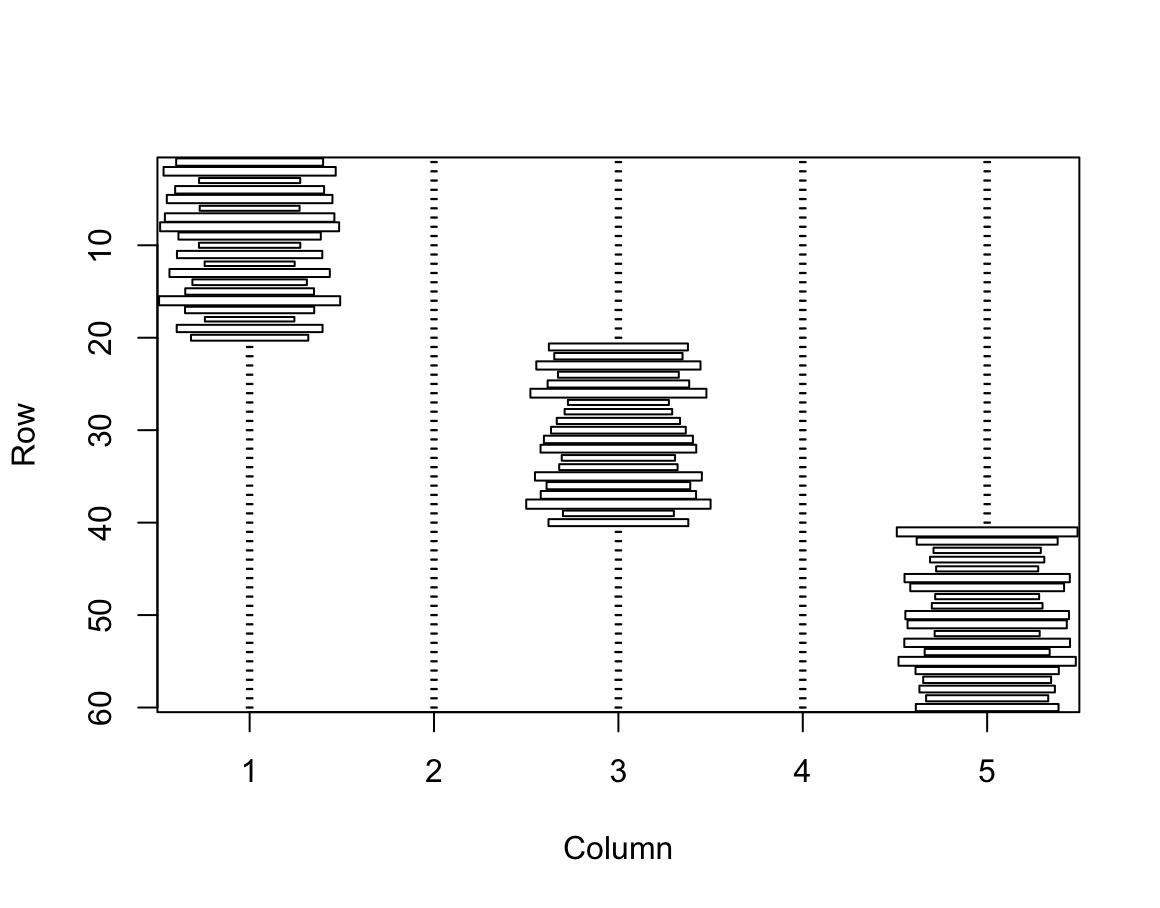
\includegraphics[width=8cm]{theta_hat.png}
	\caption{Hinton diagram for the posterior median of matrix $\Theta$, where $K=5$ latent dimensions were assumed.}
	\label{fig:theta_hat}
\end{figure}

It is instructive to examine posterior for shrinkage parameters $\beta_k$ in Figure \ref{fig:beta}: those for surplus variables are squashed towards zero.

\begin{figure}
	\centering
	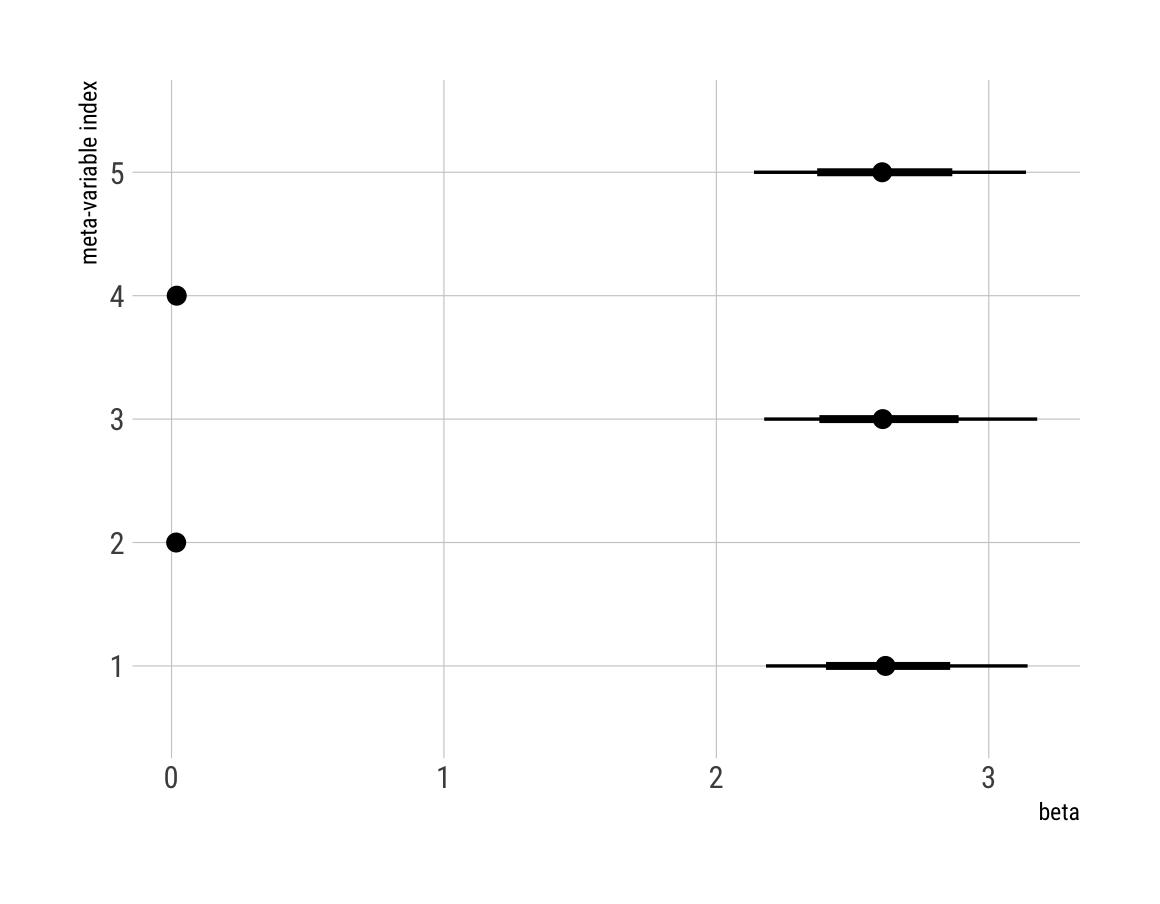
\includegraphics[width=8cm]{beta.png}
	\caption{Posterior medians (points) and $90\%$ credible intervals (segments) for shrinkage parameters $\beta_k$.}
	\label{fig:beta}
\end{figure}

Posterior median for matrix $\Theta$ can be replotted with columns arranged according to the sizes of the inferred shrinkage parameters $\beta_k$. See Figure \ref{fig:theta_hat_reordered}.

\begin{figure}
	\centering
	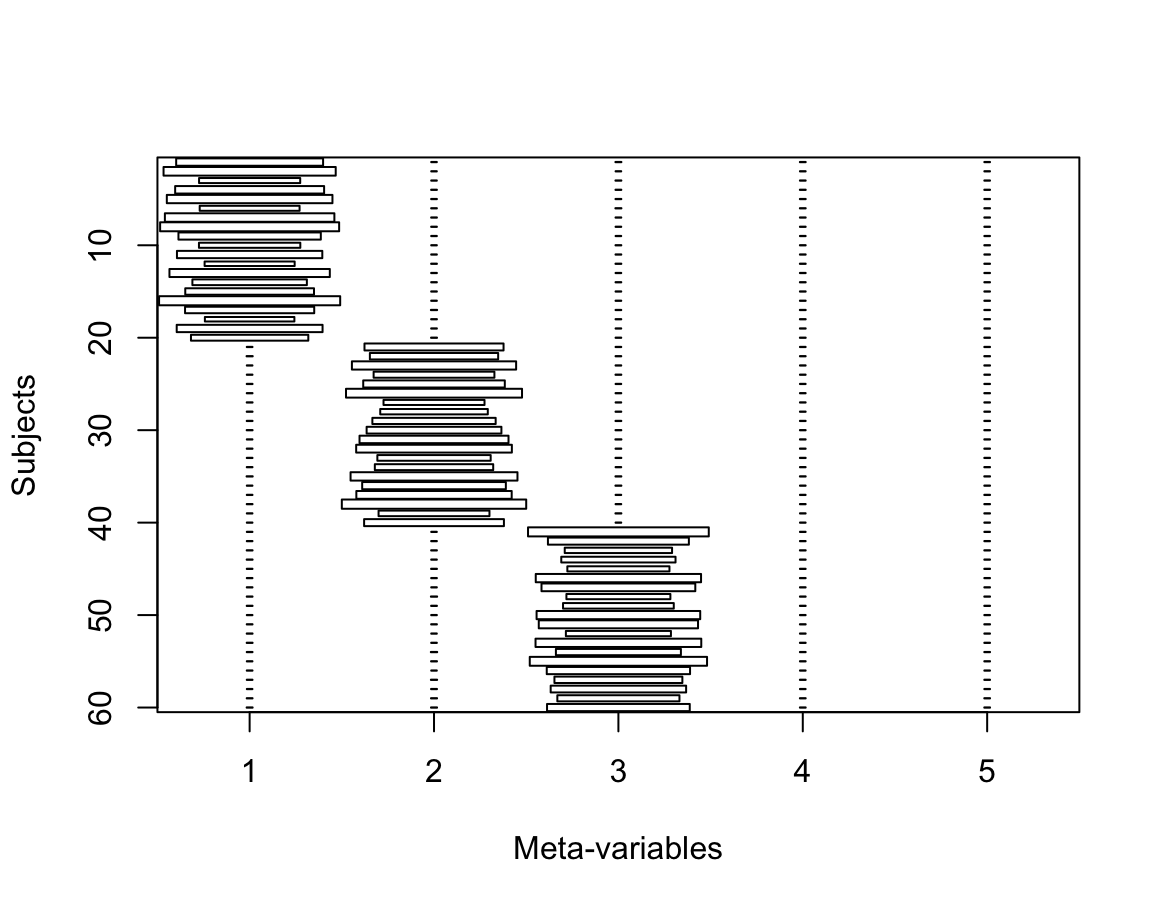
\includegraphics[width=8cm]{theta_hat_reordered.png}
	\caption{Hinton diagram for the posterior median of matrix $\Theta$, where $K=5$ latent dimensions were assumed. Columns are reordered according to the sizes of the inferred shrinkage parameters $\beta_k$.}
	\label{fig:theta_hat_reordered}
\end{figure}

The first two meta-variables are enough to discern 3 clusters in the original signal. This is clear from Figure \ref{fig:theta_hat_reordered}, but also from Figure \ref{fig:2var}.

\begin{figure}
	\centering
	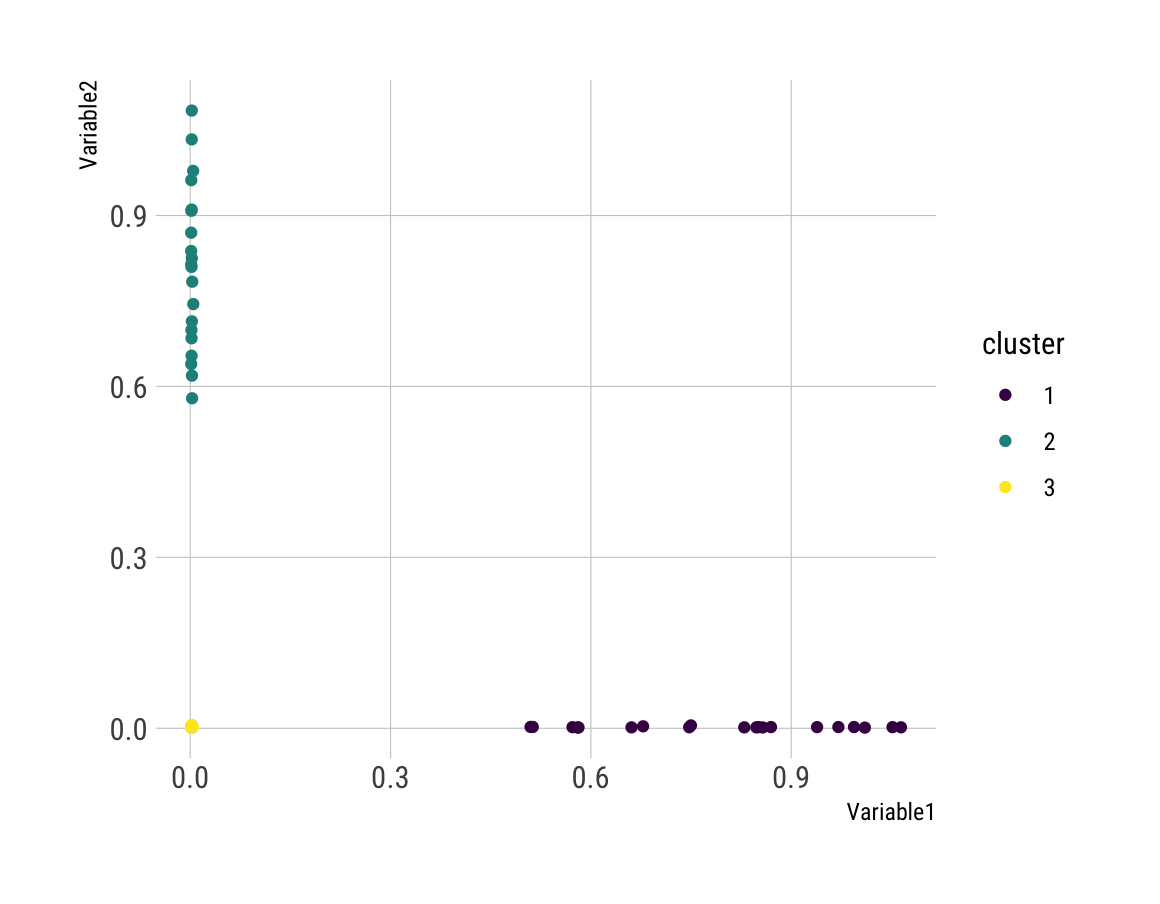
\includegraphics[width=8cm]{2var.png}
	\caption{First two latent variables according to the sizes of the inferred shrinkage parameters $\beta_k$. Points in the third cluster are visually indistinguishable from each other, as their coordinates are very small.}
	\label{fig:2var}
\end{figure}

For comparison, one can also perform PCA (via \texttt{prcomp} in {\bf R}) on the centred and scaled data matrix, retaining $5$ components, say. These 5 components explain $63\%$ of variation in data. The resulting matrix of scores is shown in Figure \ref{fig:pca_theta}. Several conclusions emerge from these plot: if the goal of the analysis were a recovery of 3 clusters in the data, then PCA performs indeed well. Thus, one cluster loads negatively the first principal component and gives low score to others, another cluster loads negatively the second principal component and gives low score to others, while the third cluster loads positively the first and second components, giving low scores to others\footnote{As noted in the corresponding {\bf R} help page, the signs returned by the decomposition may differ between different builds of {\bf R}.}. Like for Bayesian NMF, two principal components are enough to cluster data, see Figure \ref{fig:pca_2pc}. On the other hand, the original matrix $\Theta$ only had non-negative entries, and these are not be retained with PCA.

\begin{figure}
	\centering
	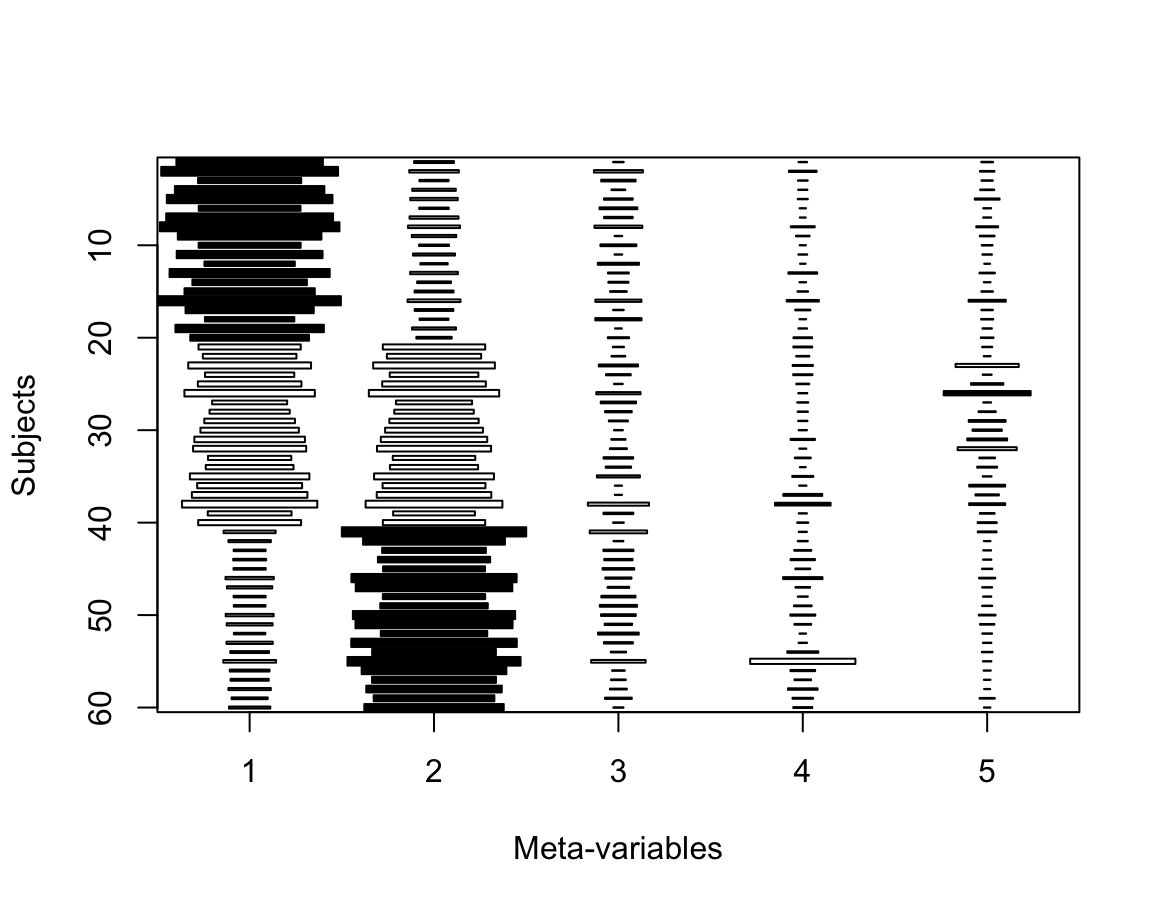
\includegraphics[width=8cm]{pca_theta.png}
	\caption{Hinton diagram for the principal components, where $K=5$ principal components have been retained.}
	\label{fig:pca_theta}
\end{figure}

\begin{figure}
	\centering
	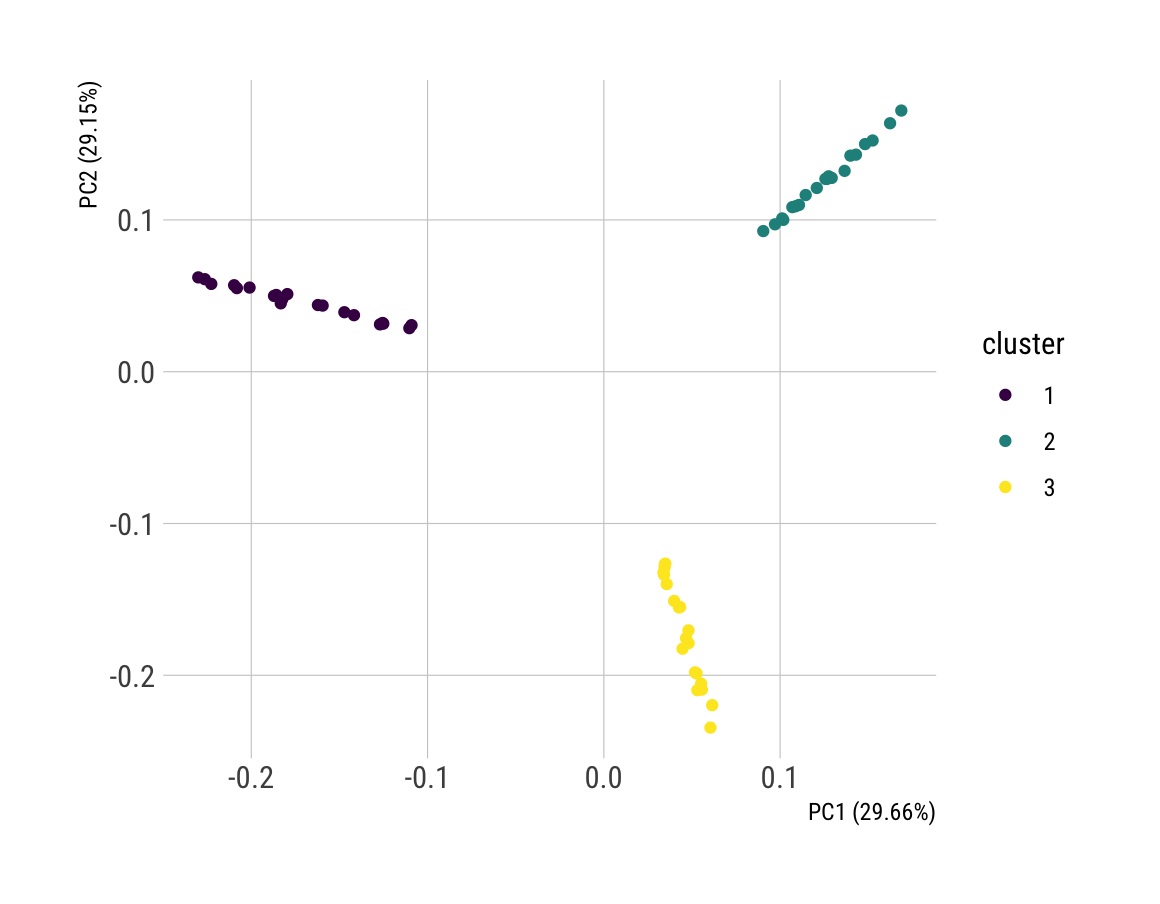
\includegraphics[width=8cm]{pca_2pc.png}
	\caption{First two principal components. Points are coloured according to clusters in the original data.}
	\label{fig:pca_2pc}
\end{figure}

Final remark concerns computational times: on a MacBook Air (2020) with Apple M1 chip with 8 cores (4 performance and 4 efficiency) and 8 GB RAM, running variational inference took just under 40 seconds. PCA was obviously massively faster. On the other hand, 40 seconds is not an impossibly long waiting time for a toy example.

\section{Apple data example}

Here is a small real data example. The dataset {\bf data.apple}, that was extracted from the supplementary materials of \citet{kumar2015}, is shipped with the {\bf R} package {\bf ASRgenomics}. It contains genotypic data on 247 apple clones (genotypes) with a total of 2,828 SNP markers (coded as 0, 1, 2, with no missing values). Genotypes were selected from 17 full-sib apple families with 25 advanced selections as parents. There were 15 genotypes per family\footnote{Thus $17 \times 15 = 247$.}.

The help page of the \texttt{snp.pca} command in {\bf ASRgenomics} analyses these data with PCA following the methodology in \citet{patterson2006} and using 10 principal components. I assumed the latter value is a reasonable starting point and fixed the dimension of the latent space at $K=10$. Only the SNP markers and no additional genetic information was used when performing the Bayesian NMF decomposition.

Posterior median for the $\Theta$ matrix is shown in Figure \ref{fig:theta_hat_apple}. The last latent variable seems to contribute little to visualisation\footnote{Whereas for Hinton diagrams I used the \texttt{color2D.matplot} command from the {\bf plotrix} package, this broke down in the present example. Therefore I switched to the heatmap, given that matrix to be plotted is much larger now. Maybe I should have done all the programming in {\bf Python}, not in {\bf R}.}.

\begin{figure}
	\centering
	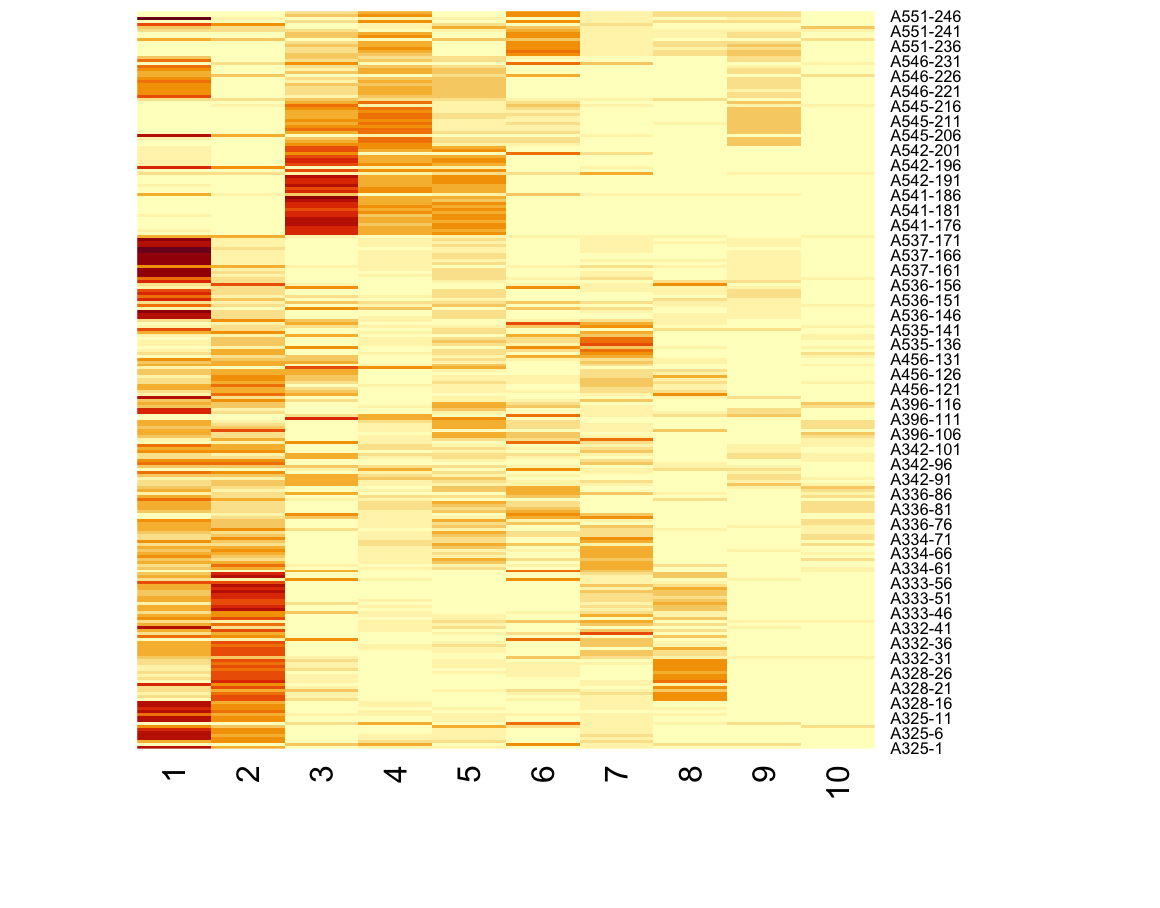
\includegraphics[width=8cm]{theta_hat_apple.png}
	\caption{Heatmap for the posterior median of matrix $\Theta$, where $K=10$ latent dimensions were assumed. Columns are reordered according to the sizes of the inferred shrinkage parameters $\beta_k$. Darker colours correspond to larger coefficients.}
	\label{fig:theta_hat_apple}
\end{figure}

As the family information is available, the Bayesian NMF results can be validated. I performed $K$-means clustering on the posterior median of ${\Theta}$ with $K=17$ cluster centres via \texttt{kmeans} in {\bf R}. The Rand score between this clustering and the truth was 0.93. Results varied slightly by choosing different random seeds, but did not go below $0.93$. One can also plot the first two latent variables with the family information superimposed, but I do not find this graph particularly useful or enlightening here. That the Bayesian NMF performed reasonably well should not be taken for granted: data are a collection of $0$, $1$ and $2$, which is not very Poisson-like, but rather more appropriate to be analysed with a binomial likelihood.

\begin{figure}
	\centering
	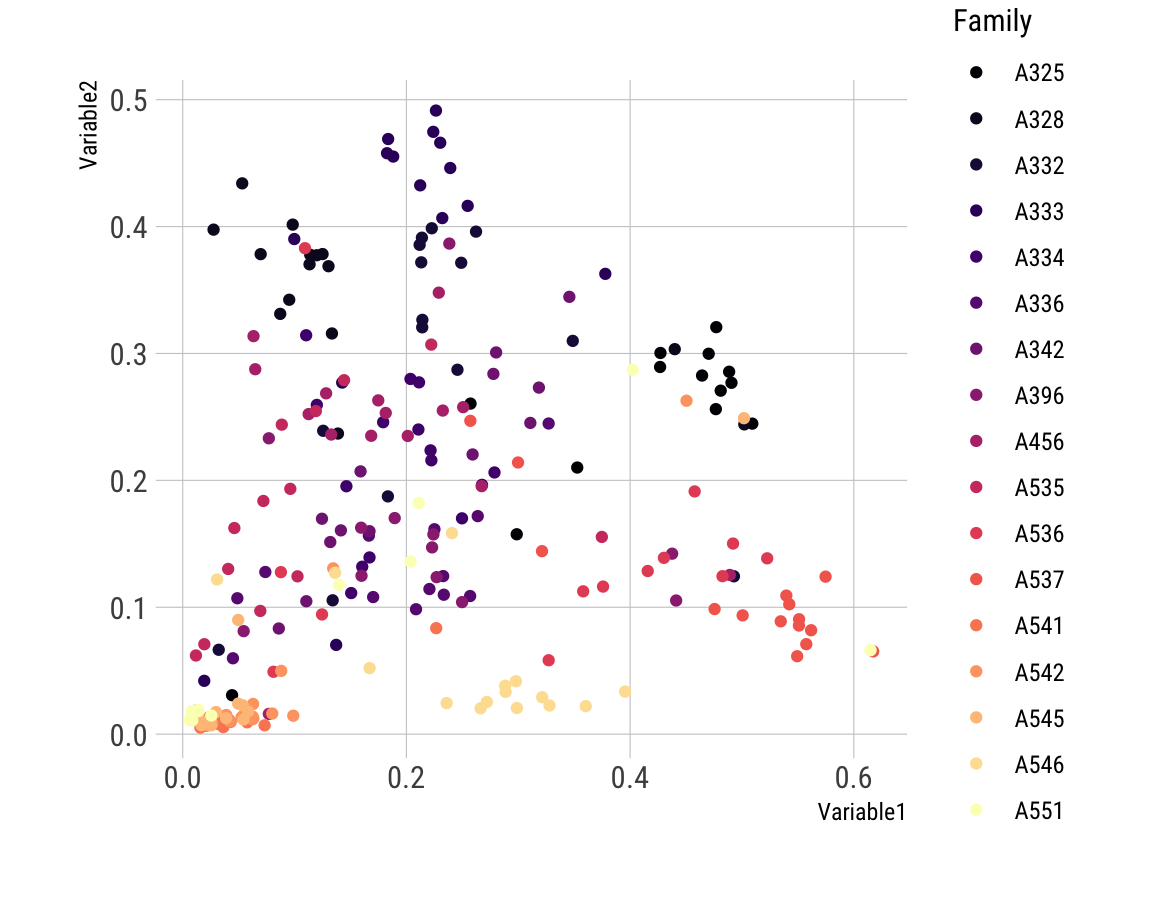
\includegraphics[width=8cm]{2var_apple.png}
	\caption{First two latent variables according to the sizes of the inferred shrinkage parameters $\beta_k$. Colours indicate families.}
	\label{fig:2var_apple}
\end{figure}

The Bayesian NMF Results can be compared to those obtained with PCA. With 10 retained principle components, the proportion of the explained variance is $85\%$. The score matrix in Figure \ref{fig:pca_scores_apple} is visually denser than the one for Bayesian NMF.

\begin{figure}
	\centering
	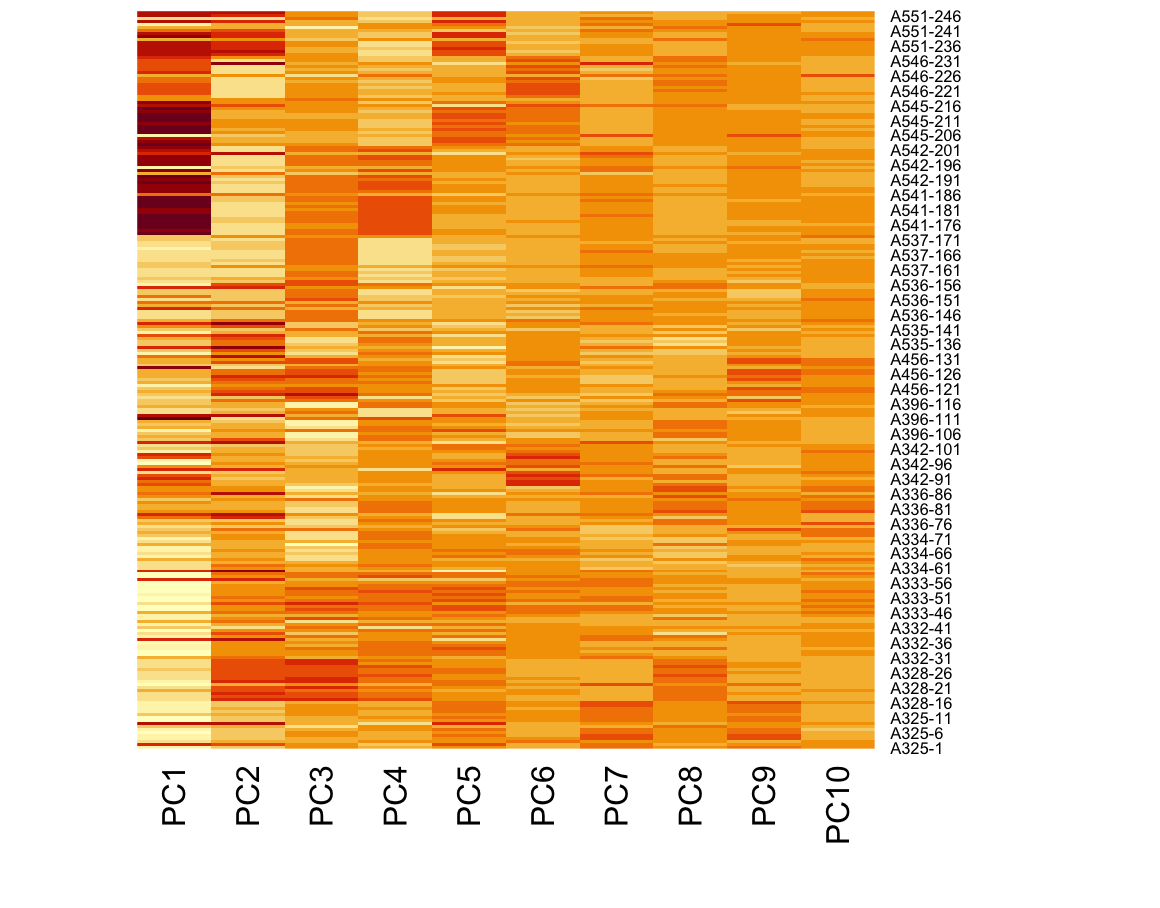
\includegraphics[width=8cm]{pca_scores_apple.png}
	\caption{Heatmap for the principal components for the PCA decomposition with $K=10$ components. Colour palette does not match that in Figure \ref{fig:theta_hat_reordered}.}
	\label{fig:pca_scores_apple}
\end{figure}

The family information can be superimposed on the plot of the first two principal components as in Figure \ref{fig:pca_families_apple}. Visually the first two components clearly identify several families, but for others the things are less clear. As already noted in \citet{kumar2015}, in almost every family there are individuals that do not cluster within their pedigree-assigned full-sib family groupings. On the other hand, the $K$-means clustering on the principal components gave the 0.93 Rand score when compared to the reference truth. This is not different from the Bayesian NMF.

\begin{figure}
	\centering
	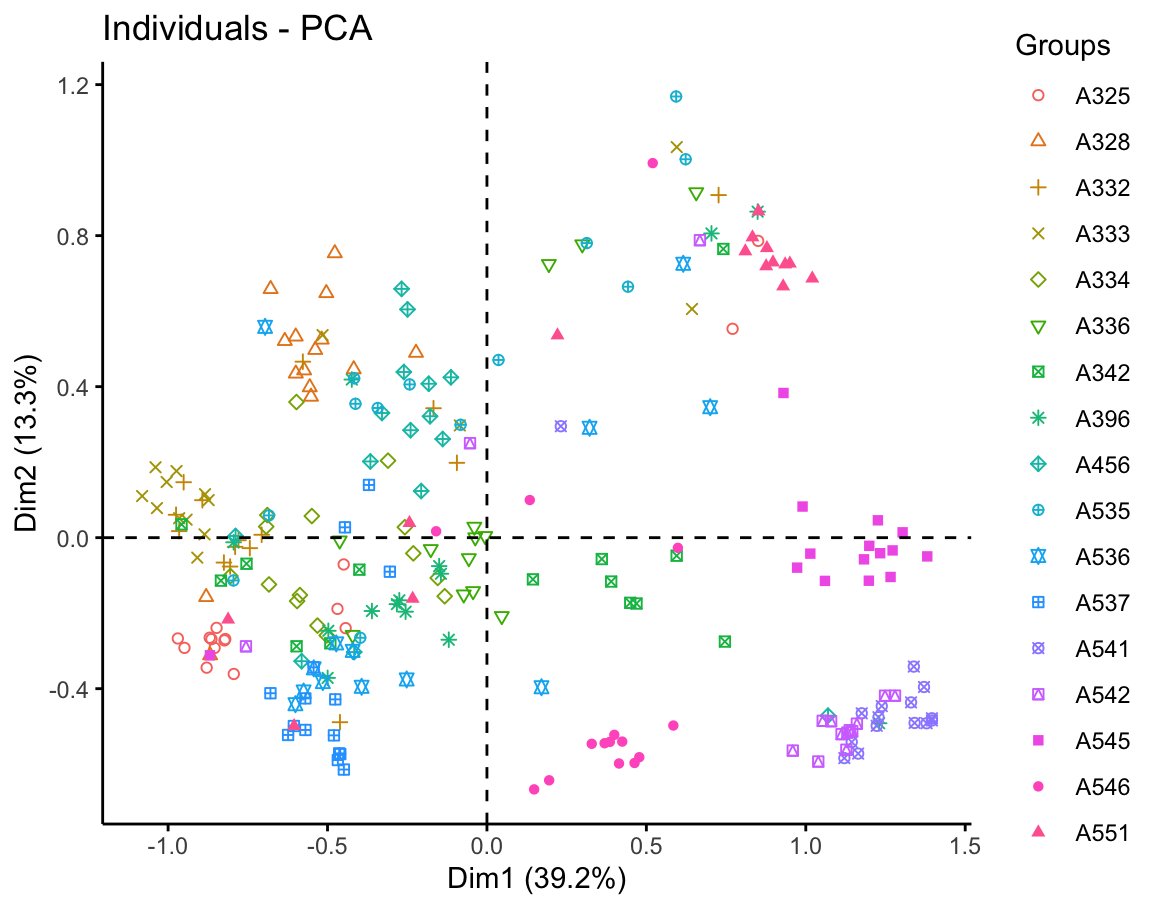
\includegraphics[width=8cm]{pca_families_apple.png}
	\caption{First two principal components. True families are indicated by different symbols.}
	\label{fig:pca_families_apple}
\end{figure}

According to \citet{venables2002}, page 316, ``Do not assume that `clustering' methods are the best way to discover interesting groupings in the data; in our experience the visualization methods are often far more effective. There are many different clustering methods, often giving different answers, and so the danger of over-interpretation is high". Here visual interpretation would have been hampered by the fact that there are 17 families. 

Final remark concerns computational times: on a MacBook Air (2020) with Apple M1 chip with 8 cores (4 performance and 4 efficiency) and 8 GB RAM, running variational inference took under 10 minute. PCA was very much faster.

\section{Recap}

NMF admits a Bayesian reformulation. This Bayesian reformulation offers some advantages over PCA as a tool for dimensionality reduction and exploratory analysis. The Bayesian NMF can be implemented through ADVI, but computationally this is more demanding than performing PCA based on SVD.

\bibliographystyle{abbrvnat}
\bibliography{notes_nmf}

\end{document}
